\chapter{Verifikation}

\section{Zeitliche Abläufe}
Vorgeben: Menge A von Aktionen
\begin{description}
\item {Ereignis (hier)} Paar bestehend aus Aktion und Zeitpunkt\\aktion(e), zeit(e) für Ereignis e.
\end{description}
Beispiel: Schlacht bei Isis 333 v. Chr. $\rightarrow$ Aktion, Zeitpunkt
\subsubsection*{Idealisierende Annahmen:}
\begin{enumerate}
\item Alles findet praktisch am selben Ort statt, keine Probleme mit der Lichtgeschwindigkeit (30cm in 1ns).
	\begin{description}
	\item[Zeit (hier)] Newtonsche Zeit, Sie verläuft
		\begin{itemize}
		\item absolut d.h. unabhängig von Beobachter (sonst: spezielle Relativitätstheorie)
		\item stetig, d.h. ohne Sprünge (sonst Quantenmechanik)
		\item unbeeinflusst von der Umgebung (sonst: allg. Relativitätstheorie)
		\item Zeitpunkt = reale Zahl
		\end{itemize}
	\end{description}
\item Ein Ereignis hat die Dauer Null. Einen Zeitraum kann man darstellen durch die Ereignisse “Ende des Zeitraums“.
\item Gleichzeitige Ereignisse sind ausgeschlossen, d.h. zwei Ereignisse, die die zur gleichen Zeit stattfinden, sind gleich\\
$zeit(e)1 = zeit(e2) \Leftrightarrow e1 = e2 $
\end{enumerate}

\begin{description}
	\item[diskreter zeitlicher Ablauf (auch Geschichte)] Menge E von Ereignissen, so dass:
	\begin{enumerate}
		\item die Menge der Zeitpunkte E keinen Häufungspunkt hat
		\item die Menge der Zeitpunkte von E ein kleinstes Element hat
	\end{enumerate}
\end{description}

Sonst: kontinuierliche Vorgänge (reaktive Systeme).\\
Interessant sind hier nicht die Zeitpunkte selber, sondern nur deren Lage zueinander, d.h. die Reihenfolge der Aktionen. (Wenn dies nicht der Fall ist und Termine eingehalten werden müssen $ \rightarrow $ Echtzeitsystem)

\begin{description}
	\item[Def: (Leslie Lamport 1978)] Ereignis $ e_1 $ kommt vor Ereignis $ e_2 $ :\\
	$ e_1 \rightarrow e_2 \Leftrightarrow \zeit(e_1) < \zeit(e_2) $
\end{description}

Beispiel: Hochmut  $ \rightarrow $ Fall.\\
Es gilt: $ \rightarrow $ ist irreflexiv, transitiv, total, fundiert (d.h. eine Wohlordnung).

Eine Relation $ R \in E \times E $ auf der Menge $ E $ heißt
\begin{labeling}{xxxxxxxxxxxxx}
	\item[irreflexiv,] falls $ \forall e \in E $ gilt: $ (e, e) \notin  R $
	\item[transitiv,] falls $ \forall e_1, e_2, e_3 \in E $ gilt: Falls $ (e_1, e_2) \in R $ und $ (e_2, e_3) \in R $, dann $ (e_1, e_3) \in R $.
	\item[total,] falls $ \forall e_1, e_2 \in E $ gilt: Falls $ e_1 \neq e_2 $, dann $(e_1, e_2) \in R $ oder $ (e_2, e_1) \in R $
	\item[fundiert,] falls es keine unendliche Folge $ (e_i)_{i \in \mathbb{N}} $ gibt mit $ e_i \in E $ für alle $ i \in \mathbb{N} $ und $ (e_i, e_{i + 1}) \in R $ für alle $ i \in \mathbb{N} $
\end{labeling}

Einschub: R azyklisch, falls es keine endliche Folge $ (e_1, ..., e_n) $ gibt mit $ (e_1, e_2) \in R, (e_2, e_3) \in R, ..., (e_{n - 1}, e_n) \in R, (e_n, e_1) \in R $.
Falls $ R $ irreflexiv und transitiv ist, dann ist $ R $ auch azyklisch.

Für einen nicht-leere Geschichte $ E $ sei $ \min \ E $ definiert als das kleinste Element von $ E $ bezüglich $ \rightarrow $, d.h. dasjenige $ e \in E $ für das gilt:

\begin{equation*}
	\forall f \in E\setminus\{e\}: e \rightarrow f
\end{equation*}

Tipp: Relation als Graph vorstellen mit Wegen.
\begin{itemize}
	\item Es existiert kein Weg der Länge 1 zu sich selber.
	\item Wenn es einen Weg von 1 zu 2 und 2 zu 3 gibt, dann existiert eine Abkürzung von 1 zu 3.
	\item Es gibt immer Weg von jedem zu jedem Knoten.
	\item Es existiert kein unendlicher Weg.
\end{itemize}

\begin{description}
	\item[Implizite Definition] Definition durch eine charakterisierende Eigenschaft.
	\item[Wohldefiniertheit der implizierten Definition] Es gibt genau ein Objekt, dass die charakterisierende Eigenschaft erfüllt.
	(Beispiel: "`Wurzel von x ist das, was quadriert x ergibt"' ist nicht eindeutig (gar keine Lösung bzw. mehrere))
\end{description}

Wohldefiniertheit von min E gilt, weil $ R $ total und E (mindestens) ein kleinstes Element hat ($ \mathbb{Z} $ sind z.B. total auf $ < $, haben aber kein kleinstes Element).

Das i-te Element aus E ($ E^i $) ist dann für $ i \in \mathbb{N}, i \leq |E| $:
\begin{equation*}
	E^i := \begin{cases}
		\min \ E & \text{falls } i = 1\\
		(E \setminus{\min \ E})^{i - 1} & \text{sonst}
	\end{cases}
\end{equation*}

Auch hier ist Wohldefiniertheit zu zeigen.\\
Projektion auf eine Menge B von Aktionen ("`Sicht"'):
\begin{equation*}
	\pi_B(E) := e \in E | aktion(e) \in B
\end{equation*}
Zustand zum Zeitpunkt $ t \in R $:
\begin{equation*}
	z_t(E) := e \in E | zeit(e) \leq t % TODO: Kleiner oder kleiner gleich?!
\end{equation*}

$ \rightarrow $ für Zeiträume: Ende von Zeitraum A kommt vor Anfang von Zeitraum B: A $ \rightarrow $ B. Es gilt: Für Zeiträume ist $ \rightarrow $ \emph{nicht} total!
$ A \rightarrow B \vee B \rightarrow A \Leftrightarrow A $ und $ B $ überlappen nicht (Wenn sich $ A $ und $ B $ überlappen gilt weder $ A  \rightarrow B $ noch $ B \rightarrow A $).

\begin{description}
	\item[Prozessalphabet] Menge der Aktionen, die der Thread p "`sieht"'
	\item[Gemeinsame Aktionen von $ p_1 $ und $ p_2 $] $ \alpha(p_1) \cap \alpha(p_2) $
	\item[Einigkeit (engl. match)] Ereignisse mit gemeinsamen Aktionen finden gemeinsam statt:
	\begin{itemize} % TODO: Besser formatieren
		\item (1) $ \pi_{\alpha(p_1) \cap \alpha(p_2)}(E_1 \cup E_2 = E_1 \cap E_2 $ Gleichwertig zu (1) sind:\\
		\item (2) $ \pi_{\alpha(p_1) \cap \alpha(p_2)}(E_1 \oplus E_2 = \emptyset $ // symmetrische Differenz: Vereinigung ohne Schnitt
		\item (3) $ \pi_{\alpha(p_1)} = \pi_{\alpha(p_2)} $
	\end{itemize}
	\item[$ E_i $ Ereignis von Thread i] Es gilt: $ \forall e \in E_i: \aktion(e) \in \alpha(p_i) $
	\item[Faire Mischung] $ E_1 \cup E_2 $
	\item[Gemeinsame Ereignisse] $ \pi_{\alpha(p_i)}(E_1 \cap E_2) = E_i, für i \in {1, 2} $, falls sich $ p_1 $ und $ p_2 $ einig sind. Es gilt: $ E_1 \cup E_2 $.
\end{description}


\section{Serielle Abläufe}
Wenn man nicht an den Zeitpunkten der Ereignisse interessiert ist, sondern nur an ihrer Lage zueinander, kann man statt einer Ereignismenge auch eine Aktionenfolge als Beschreibungsmittel für einen Ablauf nehmen.

Beispiele: Sei $ A = \{a, b\} $. Endliche Folge $ (a, b, a) $ kann auch dargestellt werden als Funktion $ f: {1, 2, 3} \rightarrow A $ mit $ f(x) = \begin{cases} a & \text{falls } x = 1 \vee x = 3\\ b & \text{sonst}\end{cases} $\\
Wertetabelle von f:
\begin{center}
	\begin{tabular}{l|c c c}
		$ x $ & 1 & 2 & 3\\ \hline
		$ f(x) $ & a & b & c
	\end{tabular}
\end{center}

Unendliche Folge $ (a, b, b, a, b, b, ...) $ als Funktion $ f: \mathbb{N} \rightarrow A $ mit $ f(x) = \begin{cases} a & \text{falls } x \mod 3 = 1\\ b & \text{sonst}\end{cases} $\\
\\
$ A^k $ k-Tupel von Elementen aus A und \\
$ {i \in \mathbb{N} | i \leq k} \rightarrow A $ Folgen der Länge k werden miteinander identifiziert.

$A^k$ k-Tupel von Elementen aus A und ${i \in \mathbb{N} | i \leq k} \rightarrow$ A Folgen der Länge k werden miteinander identifiziert.

Um endliche und unendliche Abläufe einheitlich zu modellieren, bildet man die \emph{Positionenmenge} $\mathbb{N}_\infty := \mathbb{N} \cup {\infty}$.\\
Vergleich $\leq$ auf $\mathbb{N}_\infty$ sei definiert durch
\begin{equation*}
m \leq n \Leftrightarrow (n = \mathbb{N}_0 \lor  m, n \in \mathbb{N}_0 \land m \leq n (auf \mathbb{N}_0).\\
\end{equation*}
Vergleich $m \leq n$ für m, n $\in \mathbb{N}_0$ liefert dasselbe bei $\leq$ auf $\mathbb{N}_0$ wie bei $\leq$ auf $\mathbb{N}_0$.
\\
$\le$ auf $\mathbb{N}_\infty$ sei definiert durch $m \le n \Leftrightarrow m \leq n \land m \neq n$.
Es gilt: $\le$ auf $\mathbb{N}_\infty$ ist eine Fortsetzung von $\le$ auf $\mathbb{N}_0$ und eine Wohlordnung.\\
Bemerkung: $\leq$ lässt sich weiter fortsetzen: Ordinalzahlen.\\
\\
\subsubsection*{Aktionenfolgen}
Sei A eine Aktionenmenge. Dann sei $A^* := \cup_{\substack{k \in \mathbb{N}_0}} A^k$.
$A^\infty := A^* \cup (\mathbb{N} \rightarrow A)$, wobei $A^k$ eine endliche Folge ist und $(\mathbb{N} \rightarrow A$ unendliche Folgen.
Es gilt $A^k = \cup_{\substack{k \in \mathbb{N}_\infty}} ({i \in \mathbb{N} | i \leq k} \rightarrow A)$.
Die Länge $\#_x$ einer Aktionenfolge x ist definiert durch $\#_k = \begin{cases}
\infty&\text{,falls $x \in (\mathbb{N} \rightarrow A)$}\\
k&\text{, falls $x \in A^k$}
\end{cases}$

Es gilt $\#_x \in \mathbb{N}_\infty$.

$\leq_{pre} \subseteq A^\infty \times A^\infty$ sei definiert durch $x \leq_{pre} y \Leftrightarrow \#_x \leq \#_y \land \forall 1 \leq i \leq \#_x: x(i) = y(i)$.\\
Beispiel: \\
x = (a, b, a, a)\\
y = (a, b, a, a, b, a, ...)\\
x ist ein Anfangsstück (auch Präfix, engl. prefix) von y\\
Es gilt $\leq_{pre}$ ist eine Ordnungsrelation (d.h. $\leq_{pre}$ ist reflexiv, transitiv, antisymmetrisch).
$\le_{pre} y \Leftrightarrow x \leq_{pre} y \land x \neq y$. strikter Anteil von $\leq_{pre}$
Es gilt: $\le_{pre}$ ist eine Striktordnung (d.h. irreflexiv, transitiv)
\\
\subsubsection*{Operationen auf Aktionenfolgen}
\begin{description}
	\item{rest} $A^\infty \setminus \{\varepsilon\} \rightarrow A^\infty$, wobei \{$\varepsilon$\} leere Aktionenfolge (= Aktionenfolge der Länge 0), ist definiert durch $rest(x)(i) = x(i+1)$. Es gilt: $\#_{rest(x)} = \infty$ falls $\#_x = \infty$ und $\#_{rest(x)} = \#_x - 1$ sonst
	\item {Konkatenation (Hintereinanderstellen)} von Aktionenfolgen ist definiert durch $(x \cdot y)(i) =
	\begin{cases}
	x(i) &,falls i \leq \#_x \\
	y(i-\#_x)&,sonst
	\end{cases}$. Der zweite Fall tritt nicht bei $\#_x = \infty$ auf. Es gilt: $x \cdot y = x$, falls $\#_x = \infty$.\\
	\item{Projektion} $\pi_B A^\infty \rightarrow A^\infty$ auf Aktionenmenge B ist rekursiv definiert durch:\\
\begin{equation*}
	\pi_B(x) = \begin{cases}
		\varepsilon &\text{, falls $x = \varepsilon$} \\
		x(1)\cdot \pi_B(rest(x)) &\text{, falls $0 < \#_x < \infty und x(1) \in B $}\\
		\pi_B(rest(x)) &\text{, falls $0 < \#_x < \infty und x(1) \notin B$ }\\
		sup{\pi_B(y) | y \le_{pre} x} &\text{, sonst (Supremum)}
	\end{cases}
\end{equation*}
\end{description}
Beispiel:
x = (a, b, c, a, b, c, ...)
B = {a, b}
Behauptung: $\pi_B$ = (a, b, a, b, ...)
Beweis: Es gilt $\#_x = \infty$. Damit $\pi_B(x) = sup{\pi_B(y) | y \le_{pre} x}$. \\
$y_0 := \varepsilon$ $y_0 <_{pre} x$. $\pi_B(y_0) = \varepsilon$(leere Allausage ist immer wahr, leere Folge hat keine Komponenten) \\
$y_1 := (a)$ $y_1 <_{pre} x$ $\pi_B(y_1) = (a)$
$y_2 := (a, b)$ $\pi_B(y_2) = (a, b)$
$y_3 := (a, b, c)$ $\pi_B(y_3) = (a, b)$
$y_4 := (a, b, c, a)$ $\pi_B(y_4) = (a, b, a)$
\\
Die Anzahl der Vorkommen $\#_B(x)$ von Aktionen aus der Menge B in $x \in A^{\infty}$ ist definiert durch $\#_B(x) = \#_{\pi_B(x)}$.
\\
Seien $a \in A, i \in \mathbb{N}, x \in A^{\infty}$. Dann ist die Position des i-ten Vorkommens von einer Aktion aus B in x \emph{$B^i_x$} definiert durch  $B^i_x = \#_y+1, falls y \cdot (a) \leq_{pre}x und a \in B und \#_B(y) = i - 1$.\\
Wohldefiniertheit ist hier zu zeigen.\\

\subsubsection*{Unendliche Wiederholung}
Für $x \in A^k$ ist \emph{$x^{\infty}$} definiert durch $x^{\infty}(i) = x((i-1)mod k + 1)$.\\
$(i-1)mod k + 1$ ist wie $i mod k$, außer wenn i ein Vielfaches von k ist:\\
$(i-1)mod k + 1$ liefert dann k statt 0.\\
\\
y ist ein Zustand der Aktionenfolge x (y ist Vergangenheit von x), wenn $y \leq_{pre} x$ und $\#_y \in \mathbb{N}_0$ also endlich.

\section{Faire Mischung}
$x \in (A \cup B)^\infty$ heißt eine faire Mischung (engl. fair merge) von $y \in A^\infty$ und $z \in B^\infty$, wenn gilt
\begin{equation*}
\pi_A(x) = y \text{ und } \pi_B(x) = z
\end{equation*}

Bemerkung: "`fair"' weil weder y noch z zu kurz kommen.\\
Bemerkung: Statt "`faire Mischung"' sagt man auch "`Verschränkung"' oder "`shuffle"' bei (Zeichenreihen).\\

Beispiel:\\
Sei $y = (0, 1)^\infty = (0, 1, 0, 1, 0, ...)$ und $z = (2,3)^\infty = (2, 3, 2, 3, 2, ...)$ mit $A = {0, 1}$ und $B = {2, 3}$. Dann ist $x_1 = (0, 2, 1, 3, 0, 2, 1, 3, ...)$ eine faire Mischung, weil \\
$(0,  1,  0,  1, ...) = y = \pi_A(x)$\\
$(2, 3, 2, 3, ...) = z = \pi_B(x)$\\.
Spezialfall $x_1$ heißt auch "`perfect shuffle"'.\\

Aber auch $x_2 = (2, 0, 1, 3, 2, 0, 1, 3, ...)$ faire Mischung. x braucht nicht periodisch zu sein oder y und z mit gleicher Geschwindigkeit zu behandeln.

\section{Sicherheits- und Liveness-Eigenschaften}
\begin{description}
\item {Spezifikation} Beschreibung der gewünschten Eigenschaften des Systems aus Anwendersicht
\item {Verifikation} Nachweis, dass das System seine Spezifikation erfüllt
\end{description}
Spezifikation eines sequentiellen Programms $f: Z \rightarrow Z$, wobei $Z$ die Menge der Programmzustände sei:
$pre_f(z) \Rightarrow post_f(f(z)), z \in Z$.
\begin{description}
\item {$z$} alter Zustand
\item {$f(z)$} neuer Zustand
\item {$pre_f: Z \rightarrow \mathbb{B}$} Vorbedingung
\item {$post_f: Z \rightarrow \mathbb{B}$} Nachbedingung
\end{description}

Beispiel:\\
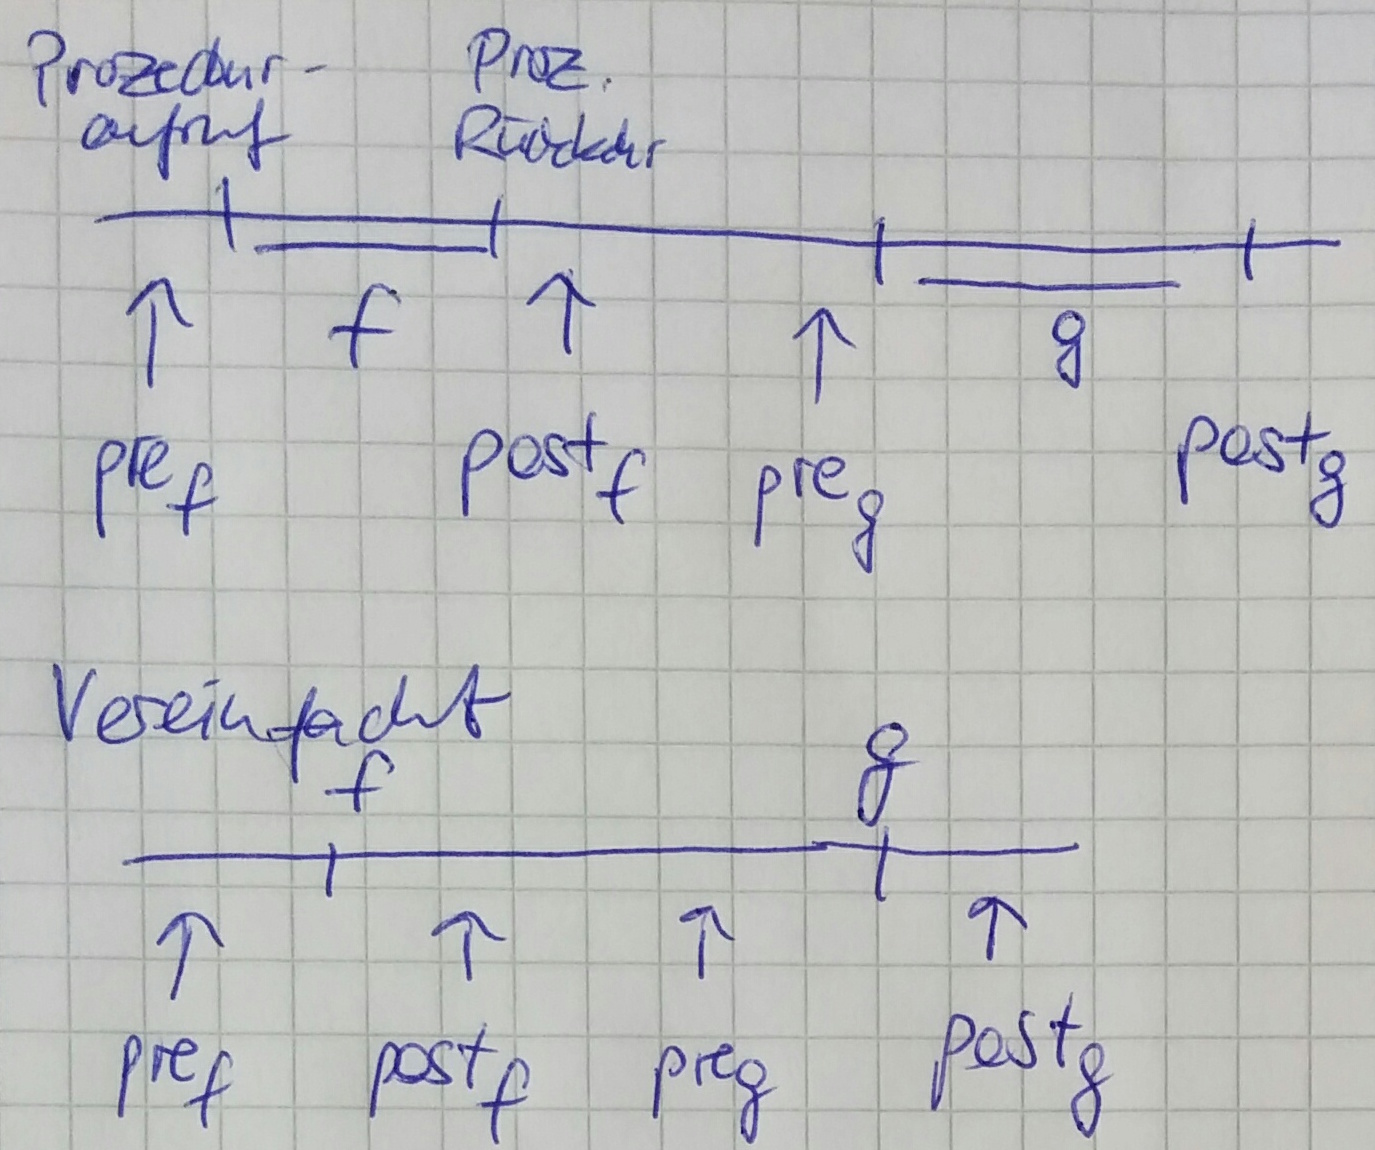
\includegraphics[width=.4\textwidth]{Verifikation_Zeitstrahl.jpeg}\\
Sequentiell: Prozedur wie einzelne Aktion behandeln\\
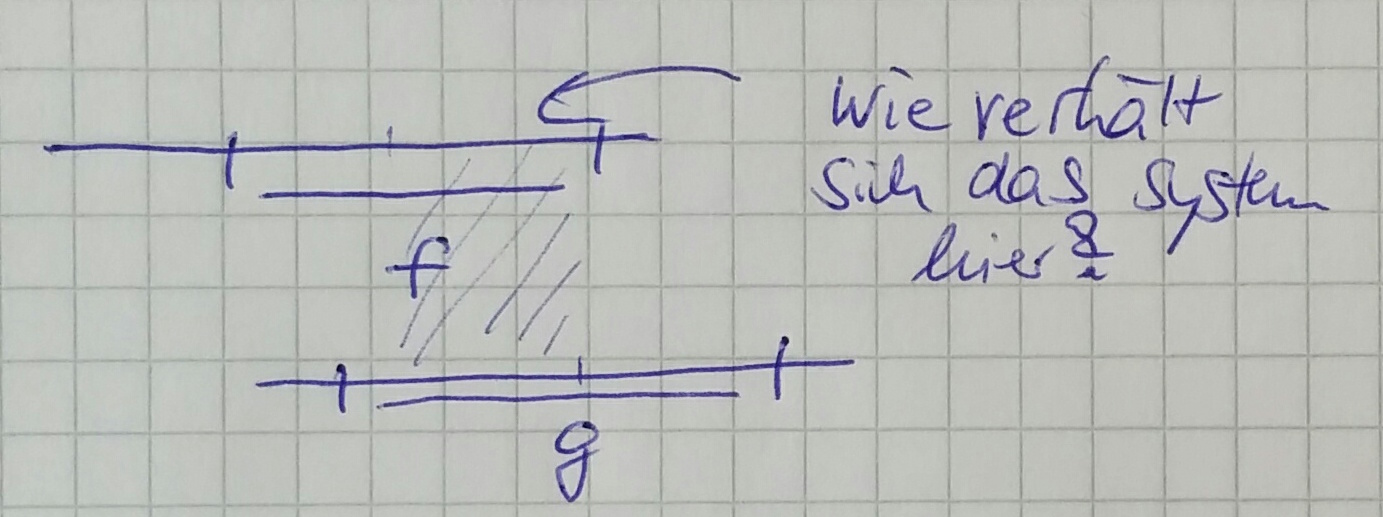
\includegraphics[width=.4\textwidth]{Verifikation_Zeitstrahl2.jpeg}\\
Problem bei Nebeneinanderablauf: siehe Zeitstrahl, Prozedurausführungen können sich überlappen. Die Ausführung von f und die Ausführung von g können sich über gemeinsame Objekt gegenseitig beeinflussen.\\
Fazit: Das Verhalten einer Prozedur f ist durch $pre_f$ und $post_f$ nicht mehr genau genug beschreibbar.\\
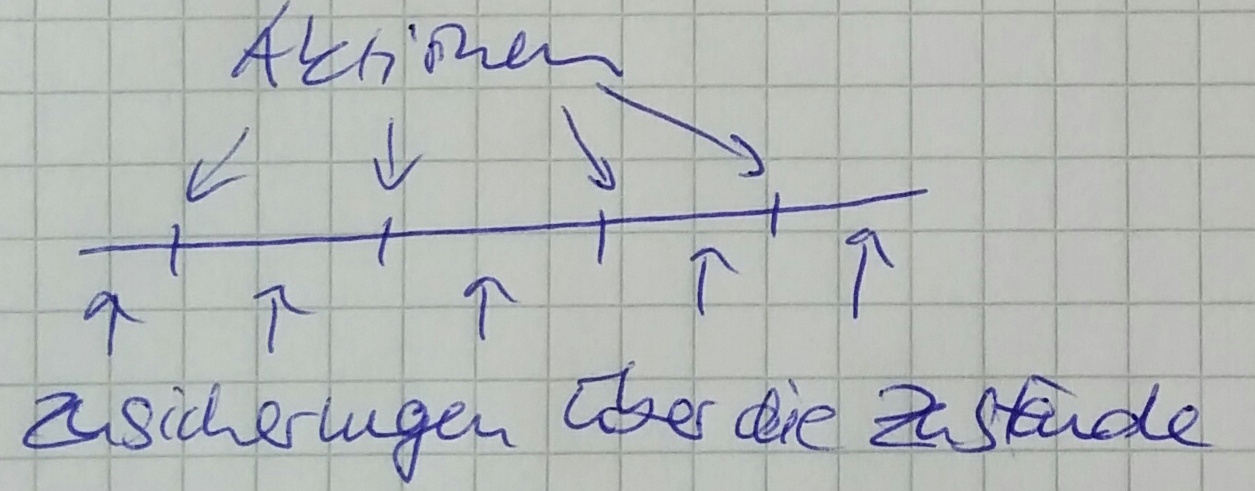
\includegraphics[width=.4\textwidth]{Verifikation_Zeitstrahl3.jpeg}\\
Vereinfachungsmöglichkeiten:\\
\begin{itemize}
\item Aktionen, die keine gemeinsamen Objekte betreffen können zusammengefasst werden zu einer Aktion
\item Kritische Bereiche können zusammengefasst werden zu einer Aktion
\end{itemize}

\begin{description}
\item {Sicherheitseigenschaft (auch: Konsistenz, Invariante, engl. safety property)} Eigenschaften, die für jeden Zustand gelten soll und die sich nur auf vergangene Zustände bezieht.
\item {Liveness-Eigenschaft (auch: Fortschritt, engl. liveness property)} alle übrigen Eigenschaften von Abläufen
\end{description}
Grund für die Unterscheidung:
\begin{enumerate}
\item Sicherheitseigenschaften sind einfacher zu beweisen.
\item Die meisten Eigenschaften sind Sicherheitseigenschaften.
\end{enumerate}
Intuitiv: Eine Sicherheitseigenschaft garantiert, dass nichts unerwünschtes geschieht ("`Verbot"'). Eine Liveness-Eigenschaft garantiert, dass \emph{schließlich} etwas Erwünschtes geschieht ("`Versprechen"'). Ein Thread, der nur wartet, erfüllt alle Sicherheitseigenschaften: "`Wer schläft, sündigt nicht"'.\\
Bemerkung: Zu sequentiellen Programmen ist partielle Korrektheit eine Sicherheitseigenschaft und Termination eine Liveness-Eigenschaft.

\subsection*{Beweismethode für eine Sicherheitseigenschaft}
"`Für jeden Zustand gilt S"':
\begin{enumerate}
\item S gilt für den Startzustand.
\item S bleibt bei jedem Zustandsübergang erhalten, d.h. wenn S im alten Zustand gilt, dann auch im neuen.
\end{enumerate}
Variante:
\begin{enumerate}
\item S gilt nach Initialisierung.
\item S bleibt außerhalb von kritischen Bereich erhalten.
\item Wenn S beim Betreten eines krit. Bereiches gilt, dann auch beim Verlassen.
\end{enumerate}
Sperren sollen folgende Eigenschaften erfüllen:
\begin{enumerate}
\item
	\begin{description}
		\item {Gegenseitiger Ausschluss} Die kritischen Bereiche zweier Threads überlappen nicht.\\Sicherheitseigenschaft: "`In jedem Zustand ist verboten, dass zwei Threads im krit. Bereich sind"'
	\end{description}
\item
	\begin{description}
		\item {Verklemmungsfreiheit} Wenn ein Thread die Sperre erwerben möchte, dann gibt es einen Thread, der die Sperre bekommt.\\
		Liveness-Eigenschaft: "`Wenn die Sperre zugeteilt werden soll, wird sie schließlich zugeteilt"'
	\end{description}
\item
	\begin{description}
		\item {Fairness (auch: kein Verhungern)} Jeder Thread, der eine Sperre erwerben möchte, bekommt sie schließlich auch.\\
	\end{description}
\end{enumerate}
Es gilt: Aus Fairness folgt Verklemmungsfreiheit.
\\
Bedingungen für Prozeduraufrufe im Zusammenhang mit nebeneinander laufenden Threads
\begin{enumerate}
\item
	\begin{description}
		\item {Bounded wait-free} Jeder Prozeduraufruf terminiert nach einer beschränkten Anzahl von Schritten.
	\end{description}
\item
	\begin{description}
		\item {Wait-free} Jeder Prozeduraufruf terminiert, d.h. bleibt nicht in einer Warteschleife hängen. (Liveness-Eigenschaft)
	\end{description}
\item
	\begin{description}
		\item {Lock-free} Unendlich viele Aufrufe terminieren. (Liveness-Eigenschaft)
	\end{description}
\end{enumerate}

\section{Modellierung}
Ausdrucksformen für Sicherheits- und Liveness-Eigenschaften:
\begin{itemize}
\item Formale Sprachen, insbesondere reguläre Ausdrücke
\item Prozessalgebra
\item Temporale Logik: linear oder verzweigend
\item Prädikatenlogik mit Abläufen als Objekten
\end{itemize}

\subsection*{Beispiel: Modellieren von Sperren}
Aktionen:
\begin{description}
	\item {$ant_i$} Thread i beantragt die Sperre
	\item {$bel_i$} Thread i belegt die Sperre (betritt den krit. Bereich)
	\item {$fr_i$} Thread i gibt die Sperre frei (verlässt den krit. Bereich)
	\item {$Bel:=\{bel_i | i \in I\}$} die Sperre wird belegt (I ist Menge der Threads)
	\item {$Fr:=\{fr_i | i \in I\}$} die Sperre wird freigegeben
\end{description}
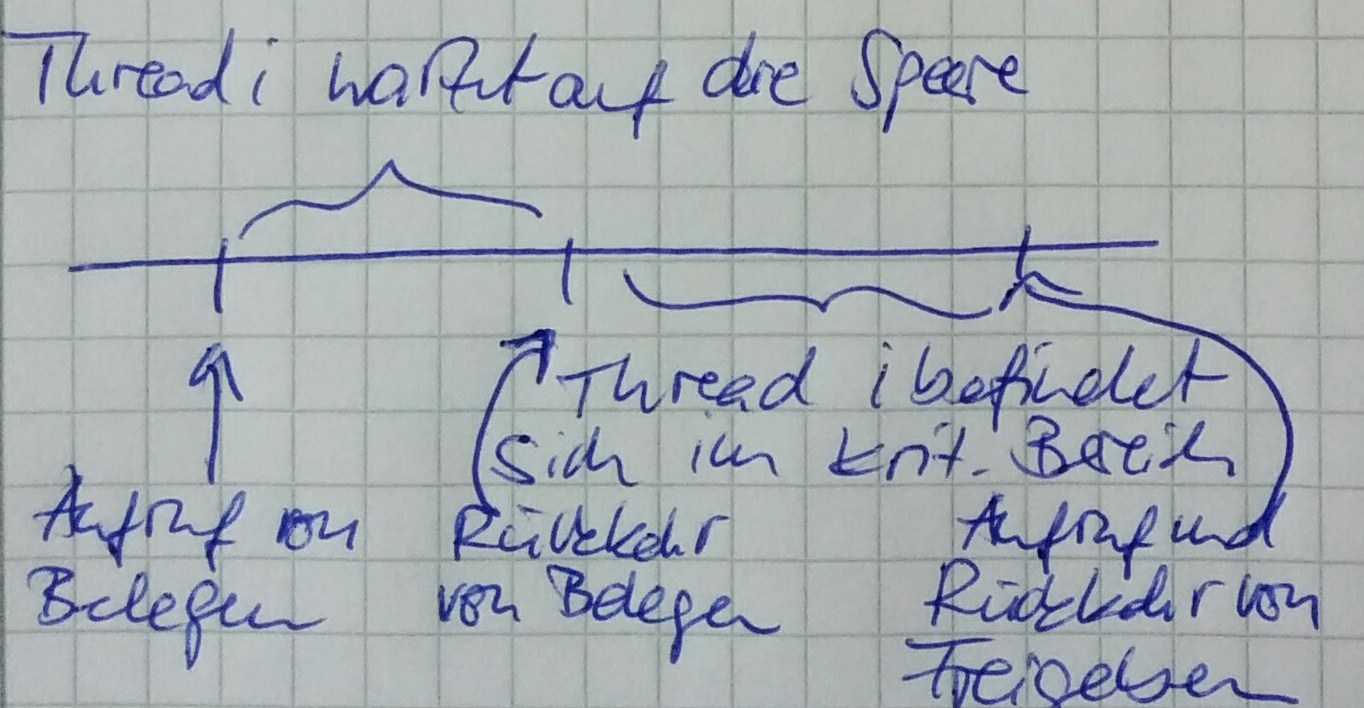
\includegraphics[width=.4\textwidth]{Verifikation_Zeitstrahl4.jpeg}\\
Gegenseitiger Ausschluss
\begin{enumerate}
	\item Mit regulären Ausdrücken\\Für jeden Ablauf x gilt: Für jedes endliche Anfangsstück y von x gilt:\\
	Die Projektion von y auf die Aktionenmenge $Bel \cup Fr$ ist in der Sprache $(Bel Fr)^*(Bel + \epsilon) = PRE((Bel Fr)^*)$ ("`Präfixabschluss"')\\
	Sei $Ant:=\{ant_i | i \in I\}$ und $A:=Ant \cup Bel \cup Fr$. Dann kann man gegenseitigen Ausschluss als Formel angeben: $\forall x \in A^{infty}: \forall y \leq_{pre} x: \#_y <_\infty \Rightarrow \pi_{Bel \cup Fr}(y) \in PRE((Bel Fr)^*)$ Ausgeschlossen ist z.B. der Ablauf $bel_1 bel_1 fr_2$\\
	Präfixablauf definiert durch $PRE(x)= \{y \in A^* | y \leq_{pre} x \}$.
\end{enumerate}

Bemerkung: Sicherheitseigenschaften kann man immer mit Präfixabschluss beweisen.